\section*{Supplementary material: verb-level transport calibration}
\addcontentsline{toc}{section}{Supplementary material: verb-level transport calibration}

Figure~\ref{fig:bnc-calibration} gives the verb-level detail behind the
reliability diagram in the main text (Figure~\ref{fig:bnc-reliability}). It
compares observed NP recipient rates with the transported source model's mean
predictions and with the BNC2014-trained model's, verb by verb, on the same
complete-case rows.

\begin{figure}[htbp]
\centering
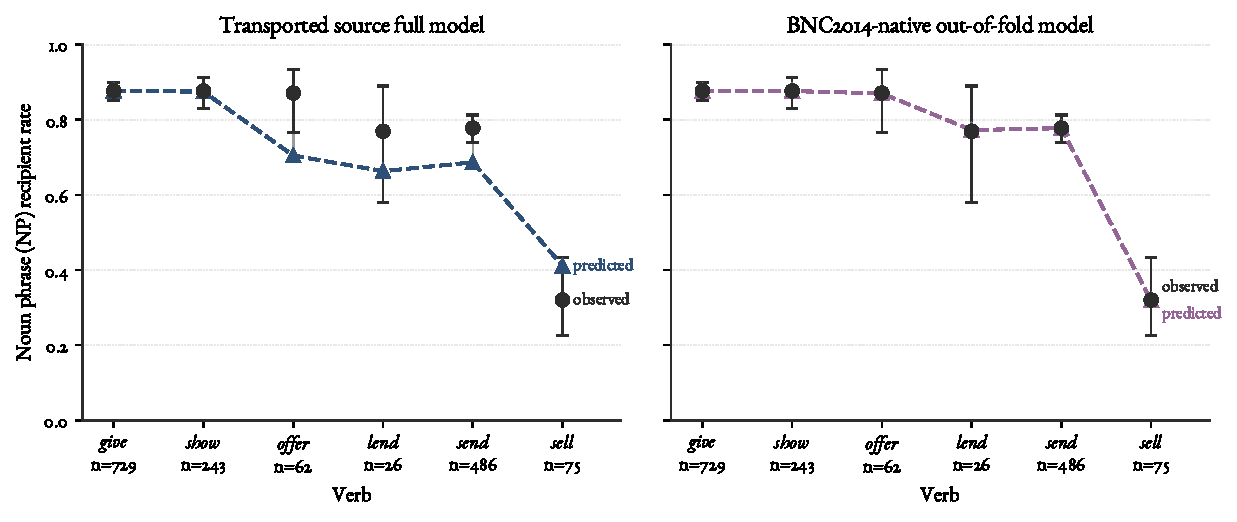
\includegraphics[width=\linewidth]{data/derived/figures/bnc2014_transport_calibration_by_verb.pdf}
\caption{Verb-level calibration for the transported source full model and the
BNC2014-trained held-out model on the same complete-case rows. Black points and
intervals are observed NP recipient rates with binomial Wilson intervals,
unadjusted for conversational clustering; coloured triangles are mean
predictions.}
\label{fig:bnc-calibration}
\end{figure}

\section*{Supplementary material: the DAIS comparative-preference bridge}
\addcontentsline{toc}{section}{Supplementary material: the DAIS comparative-preference bridge}

DAIS asks a neighbouring question: when participants see double-object and
prepositional-object versions of the same constructed item, do their preferences
follow the corpus model's production probabilities? This bridge is supplementary
to the external-validation result and is reported for completeness rather than
as part of the paper's main claim.

The Dative Alternation and Information Structure (DAIS) dataset,
introduced by
\textcite{HawkinsYamakoshiGriffithsGoldberg2020VerbBias}, contains 50,000 human
judgements over 5,000 dative sentence pairs and systematically varies verb,
definiteness, and argument length. Participants saw both variants of each pair
together and used a slider to indicate their relative preference for the
double-object (DO) variant over the prepositional-object (PO) variant, with the
midpoint labelled \enquote{about the same}. DAIS gives comparative
preference conditioned on a pair, not an absolute acceptability rating of an
individual sentence. The repository carries a CC BY 4.0 licence, and the
dataset authors have given explicit permission to reuse the judgements, so DAIS
can enter as a compact bridge
\citep{HawkinsYamakoshiGriffithsGoldberg2020DAIS}.

The bridge keeps the targets separate. I score only the 150 DAIS items whose
verbs overlap the six-verb production core. The transported spoken
\texttt{languageR} model gives each constructed pair an NP-recipient production
probability. The DAIS item mean gives the corresponding human paired DO
preference, preference for the same NP-recipient form over its PO counterpart,
on a 0--1 scale. Those two values measure different quantities: conditional
realization among attested corpus tokens and pairwise slider preference in
constructed items. The bridge asks whether they rank items similarly, and where
they depart after marginal calibration.

The cleaned DAIS responses use integer values from 0 to 100 and are scaled here
by division by 100. The shared-verb subset contains 1,525 judgement rows from
923 participants over 150 constructed items. Item support ranges from 6 to 14
judgements, with a median of 10; the mean item-level standard error is 0.082 on
the 0--1 response scale.

\begin{figure}[htbp]
\centering
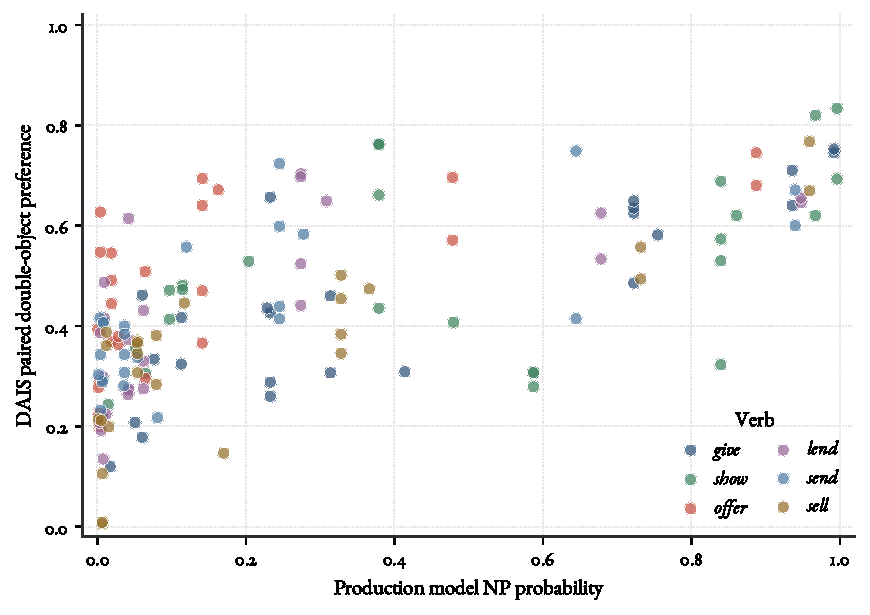
\includegraphics[width=0.82\linewidth]{data/derived/figures/dais_production_preference_bridge.pdf}
\caption{DAIS production/preference bridge for the six shared verbs. Each point
is a constructed DAIS item. The horizontal axis is the spoken
\texttt{languageR} model's NP recipient probability; the vertical axis is DAIS
paired DO preference. No equality line is shown because the axes are different
measurement scales: corpus production probability and comparative slider
preference. Points are coloured by verb.}
\label{fig:dais-bridge}
\end{figure}

\begin{table}[htbp]
\centering
\small
\begin{tabular}{lrrr}
\toprule
Verb & Prod. rank & DAIS rank & Calib. resid. \\
\midrule
\mention{show} & 1 & 1 & -0.005 \\
\mention{give} & 2 & 3 & -0.036 \\
\mention{sell} & 3 & 6 & -0.070 \\
\mention{lend} & 4 & 5 & 0.015 \\
\mention{send} & 5 & 4 & 0.020 \\
\mention{offer} & 6 & 2 & 0.077 \\
\bottomrule
\end{tabular}
\caption{DAIS bridge for the six shared verbs. Ranks order verbs from strongest
to weakest NP/DO preference within each channel. The residual column is mean
DAIS paired preference after marginal calibration on production probability;
positive values mean more DO preference than the marginal production--preference
relation predicts.}
\label{tab:dais-bridge}
\end{table}

The two channels line up moderately, while remaining distinct. With
\mention{something} treated as a pronominal theme, Pearson's \(r\) is 0.667 and
Spearman's \(\rho\) is 0.685 over the 150 shared-verb items. Treating
\mention{something} as nonpronominal gives the same rank-based interpretation
(\(r = 0.645\), \(\rho = 0.675\)). The raw difference between the
production-probability level and the DAIS slider level would be a misleading
absolute calibration error, because the midpoint-labelled comparative scale
compresses item means toward 0.5 and uses a different measurement scale from a
corpus production probability.

The item and participant checks show why the raw correlation needs a cautious
reading. At the item level, a marginal calibration regression has a positive
slope, but once recipient condition, theme type, and verb are represented
directly, the production-score slope is essentially zero (0.006, standard error
0.078).

A judgement-level mixed model gives the same caution. It predicts the scaled
comparative slider response from production score, recipient condition, theme
type, and verb, with random intercepts for participant and constructed item. The
incremental production-score coefficient is 0.017 (standard error 0.076;
approximate interval \([-0.132,0.165]\)). DAIS preference and production
probability show moderate marginal rank correspondence, much of it attributable
to shared sensitivity to the manipulated predictors; the production score adds
little once those predictors are represented directly.

The useful cases are calibrated divergences, not isolated raw gaps. After a
marginal production--preference calibration, the verb-level residual is 0.077
for \mention{offer} (bootstrap interval 0.027 to 0.129) and \(-0.070\) for
\mention{sell} (interval \(-0.119\) to \(-0.027\)). The point is channel
separation: two comparative measures defined over the same alternation frame
can preserve moderate rank correspondence while still disagreeing in
calibrated, verb-specific ways.
